\documentclass[11pt]{article}
\usepackage[sort]{natbib}
\usepackage{bm,amsmath,bbm,amsfonts,nicefrac,latexsym,amsmath,amsfonts,amsbsy,amscd,amsxtra,amsgen,amsopn,bbm,amsthm,amssymb,graphicx}
\usepackage{fancyhdr, subcaption}
\usepackage[margin=1.0in]{geometry}
\usepackage[section]{placeins}
\bibliographystyle{abbrvnat}

\title{Data chapter}
\author{Ewan Pinnington}

\newtheorem{theorem}{Theorem}[section]
\newtheorem*{defn}{Definition}


\begin{document}

\maketitle

\section{Introduction}

As part of this PhD an extended period of time has been spent at the Alice Holt Research Station (Hampshire, UK) working with Forest Research (The research arm of the UK Forestry Commission). After initially completing one year of an ongoing field campaign to measure stem respiration using an infra-red gas analyser, a measurement campaign was designed to produce a set of observations for use in this PhD project. This involved the establishment and sampling of three transects throughout the Straits Inclosure (part of the Alice Holt forest). The establishment of these transect and measurements are outlined in this chapter.


\section{Alice Holt research site}

The Alice Holt Forest is a research forest area managed by the UK Forestry Commission located in Hampshire, SE England. Forest Research have been operating a $\text{CO}_{2}$ flux measurement tower in a portion of the forest, the Straits Inclosure, continuously since 1998. The Straits Inclosure is a $90~\text{ha}$ area of deciduous broadleaved plantation woodland located on a surface water gley soil and was initially planted with oak in the 1820s \citep{schlich1905working} and then replanted in the 1930s. The majority of the canopy trees are oak (\textit{Quercus robur} L.), with an understory of hazel (\textit{Corylus avellana} L.) and hawthorn (\textit{Crataegus monogyna} Jacq.) \citep{pitman2001leaf}, but there is a small area of conifers (\textit{Pinus nigra} ssp. \textit{laricio} (Maire) and \textit{P. sylvestris} L.) within the tower measurement footprint area depending on wind direction. An aerial photograph of the site is shown in Figure~\ref{fig:ah_aerial_photo}. The Straits Inclosure is a flat area at an altitude of approximately 80m, surrounded by mixed lowland woods and both arable and pasture agricultural land. In \citet{wilkinson2012inter} an analysis of stand-scale $30$ minute average net $\text{CO}_{2}$ fluxes (NEE) from 1998-2011 for the Straits Inclosure found a mean annual NEE of \(-486~\text{g C m}^{-2}~\text{yr}^{-1}\) and demonstrated the forest was a substantial sink of carbon. This study also includes further details about the research site. 

As part of the management regime, the Straits Inclosure is subject to thinning, whereby a proportion of trees are removed from the canopy in order to reduce competition and improve the quality of the final tree crop. At the Straits an intermediate thinning method is used with a portion of both subdominant and dominant trees being removed from the stand \citep{kerr2011thinning}. The whole of the stand was thinned in 1995. Subsequently the eastern side of the Straits was thinned in 2007 and then the western side in 2014. The flux tower at the site is situated on the boundary between these two sides. This allows for the use of a footprint model to split the flux record and thus analyse the effect of this disturbance on carbon fluxes at the site. In \citet{wilkinson2015effects} a statistical analysis of the eddy covariance flux record found that there was no significant effect on the net carbon uptake of the eastern side after thinning in 2007. In this thesis we focus on the effect of disturbance on the western side after thinning in 2014 in chapter REF. We therefore refer to the western side as ``thinned'' forest and the eastern side as ``unthinned'' forest.   


\begin{figure}[ht]
    \centering
    \includegraphics[width=0.8\textwidth]{AP1_2013.jpg}
    \caption{The Straits Inclosure research site in 2013.} \label{fig:ah_aerial_photo}
\end{figure}

\section{Establishment of sampling points}

For this fieldwork transects were designed to join up existing mensuration plots where measurements of woody biomass are made by Forest Research. This would then allow for comparison with historic observations. In total 435 sampling points were marked at 10m intervals, these are shown in Figure~\ref{fig:transects}. Python was used to calculated the exact latitude and longitude of each sampling point for the 3 transects, these locations were then entered into a GPS unit. When establishing the transects fluorescent spray paint was used to mark trees closest to each sampling point as shown on the GPS (see Figure~\ref{fig:pink_tree}). As parts of the forest site were extremely dense with vegetation a pair of loppers were used to clear a path in some areas to allow for the construction of relatively straight transects. Having all transect points numbered and corresponding to a latitude and longitude value allowed for comparison between methods and the splitting of observations between different distinct sections of the forest site. 


\begin{figure}[ht]
    \centering
    \includegraphics[width=\textwidth]{straitsmap_threet_10m.png}
    \caption{Sampling transects. Black crosses: sampling points at 10m intervals, pink diamonds: Forest Research mensuration plots, black diamond: Forest Research flux tower.} \label{fig:transects}
\end{figure}

\begin{figure}[ht]
    \centering
    \includegraphics[width=0.8\textwidth]{291E.jpg}
    \caption{Sampling point 291, showing fluorescent spray paint used to mark sampling points.} \label{fig:pink_tree}
\end{figure}

\section{Leaf area index observations}

The Leaf Area Index (LAI) is an important variable in relation to the amount of CO2 an ecosystem can remove from the atmosphere through photosynthesis. LAI can be thought of as the area of leaves per unit area of ground. Three different methods were used to measure LAI along the three transects at different sampling intervals. 

\subsection{Ceptometer}

A ceptometer and an additional Photosynthetically Active Radiation (PAR) sensor were used to measure LAI. Here we measure below canopy PAR using the ceptometer while logging above canopy PAR using a data logger and PAR sensor positioned outside the canopy. We can then calculate LAI using the above and below canopy readings and a set of equations relying on some assumptions \citep{fassnacht1994comparison}. The ceptometer represents the quickest method for estimating LAI, we therefore took readings with the ceptometer at every sampling point over two walks of the transects, giving us 870 observations in total.

In order to be sure that the PAR readings from the ceptometer and external PAR sensor were consistent we had to calibrate the PAR sensor against the ceptometer. This was done by leaving both the PAR sensor and ceptometer out logging next to each other every 10 seconds for a day in the Alice Holt Research Station met square. We can then calibrate he output of the PAR sensor with that of the ceptometer as shown in Figure~\ref{fig:par_calib}. 

\begin{figure}[ht]
    \centering
    \includegraphics[width=0.8\textwidth]{AH_PAR.pdf}
    \caption{Calibration of above canopy Photosynthetically Active Radiation (PAR) sensor (measuring in mV) with LP-80 ceptometer measured PAR (\(\mu \text{mol}~\text{m}^{-2}~\text{s}^{-1} \)).} \label{fig:par_calib}
\end{figure}

Once the PAR sensor was calibrate measurements could be made along the transects. The PAR sensor positioned outside of the canopy was logged every 5 seconds using a Decagon DL2e data logger, at the start of every set of measurements the clock on the data logger and ceptometer were synchronised to ensure comparison of measurements made at the same time. After sampling the transects we had a set of above canopy and below canopy PAR readings corresponding to each sampling point for both walks of the transects. These readings were then used in the following equations to estimate LAI:

EQUATIONS!!!

We then took the mean of the two LAI observations at each point to give as an estimate to the peak LAI for the year 2015. We can see the LAI estimate for the Straits Inclosure in Figure~\ref{fig:cept_lai}. 

\begin{figure}[ht]
    \centering
    \includegraphics[width=0.8\textwidth]{lai_cept.pdf}
    \caption{Ceptometer derived LAI for Alice Holt.} \label{fig:cept_lai}
\end{figure}

\subsection{Hemispherical photographs}

\begin{figure}[ht]
\centering
\begin{subfigure}{.5\textwidth}
  \centering
  \includegraphics[width=.9\linewidth]{043exp2.jpg}
  \caption{Unthinned forest}
  \label{fig:sub1}
\end{subfigure}%
\begin{subfigure}{.5\textwidth}
  \centering
  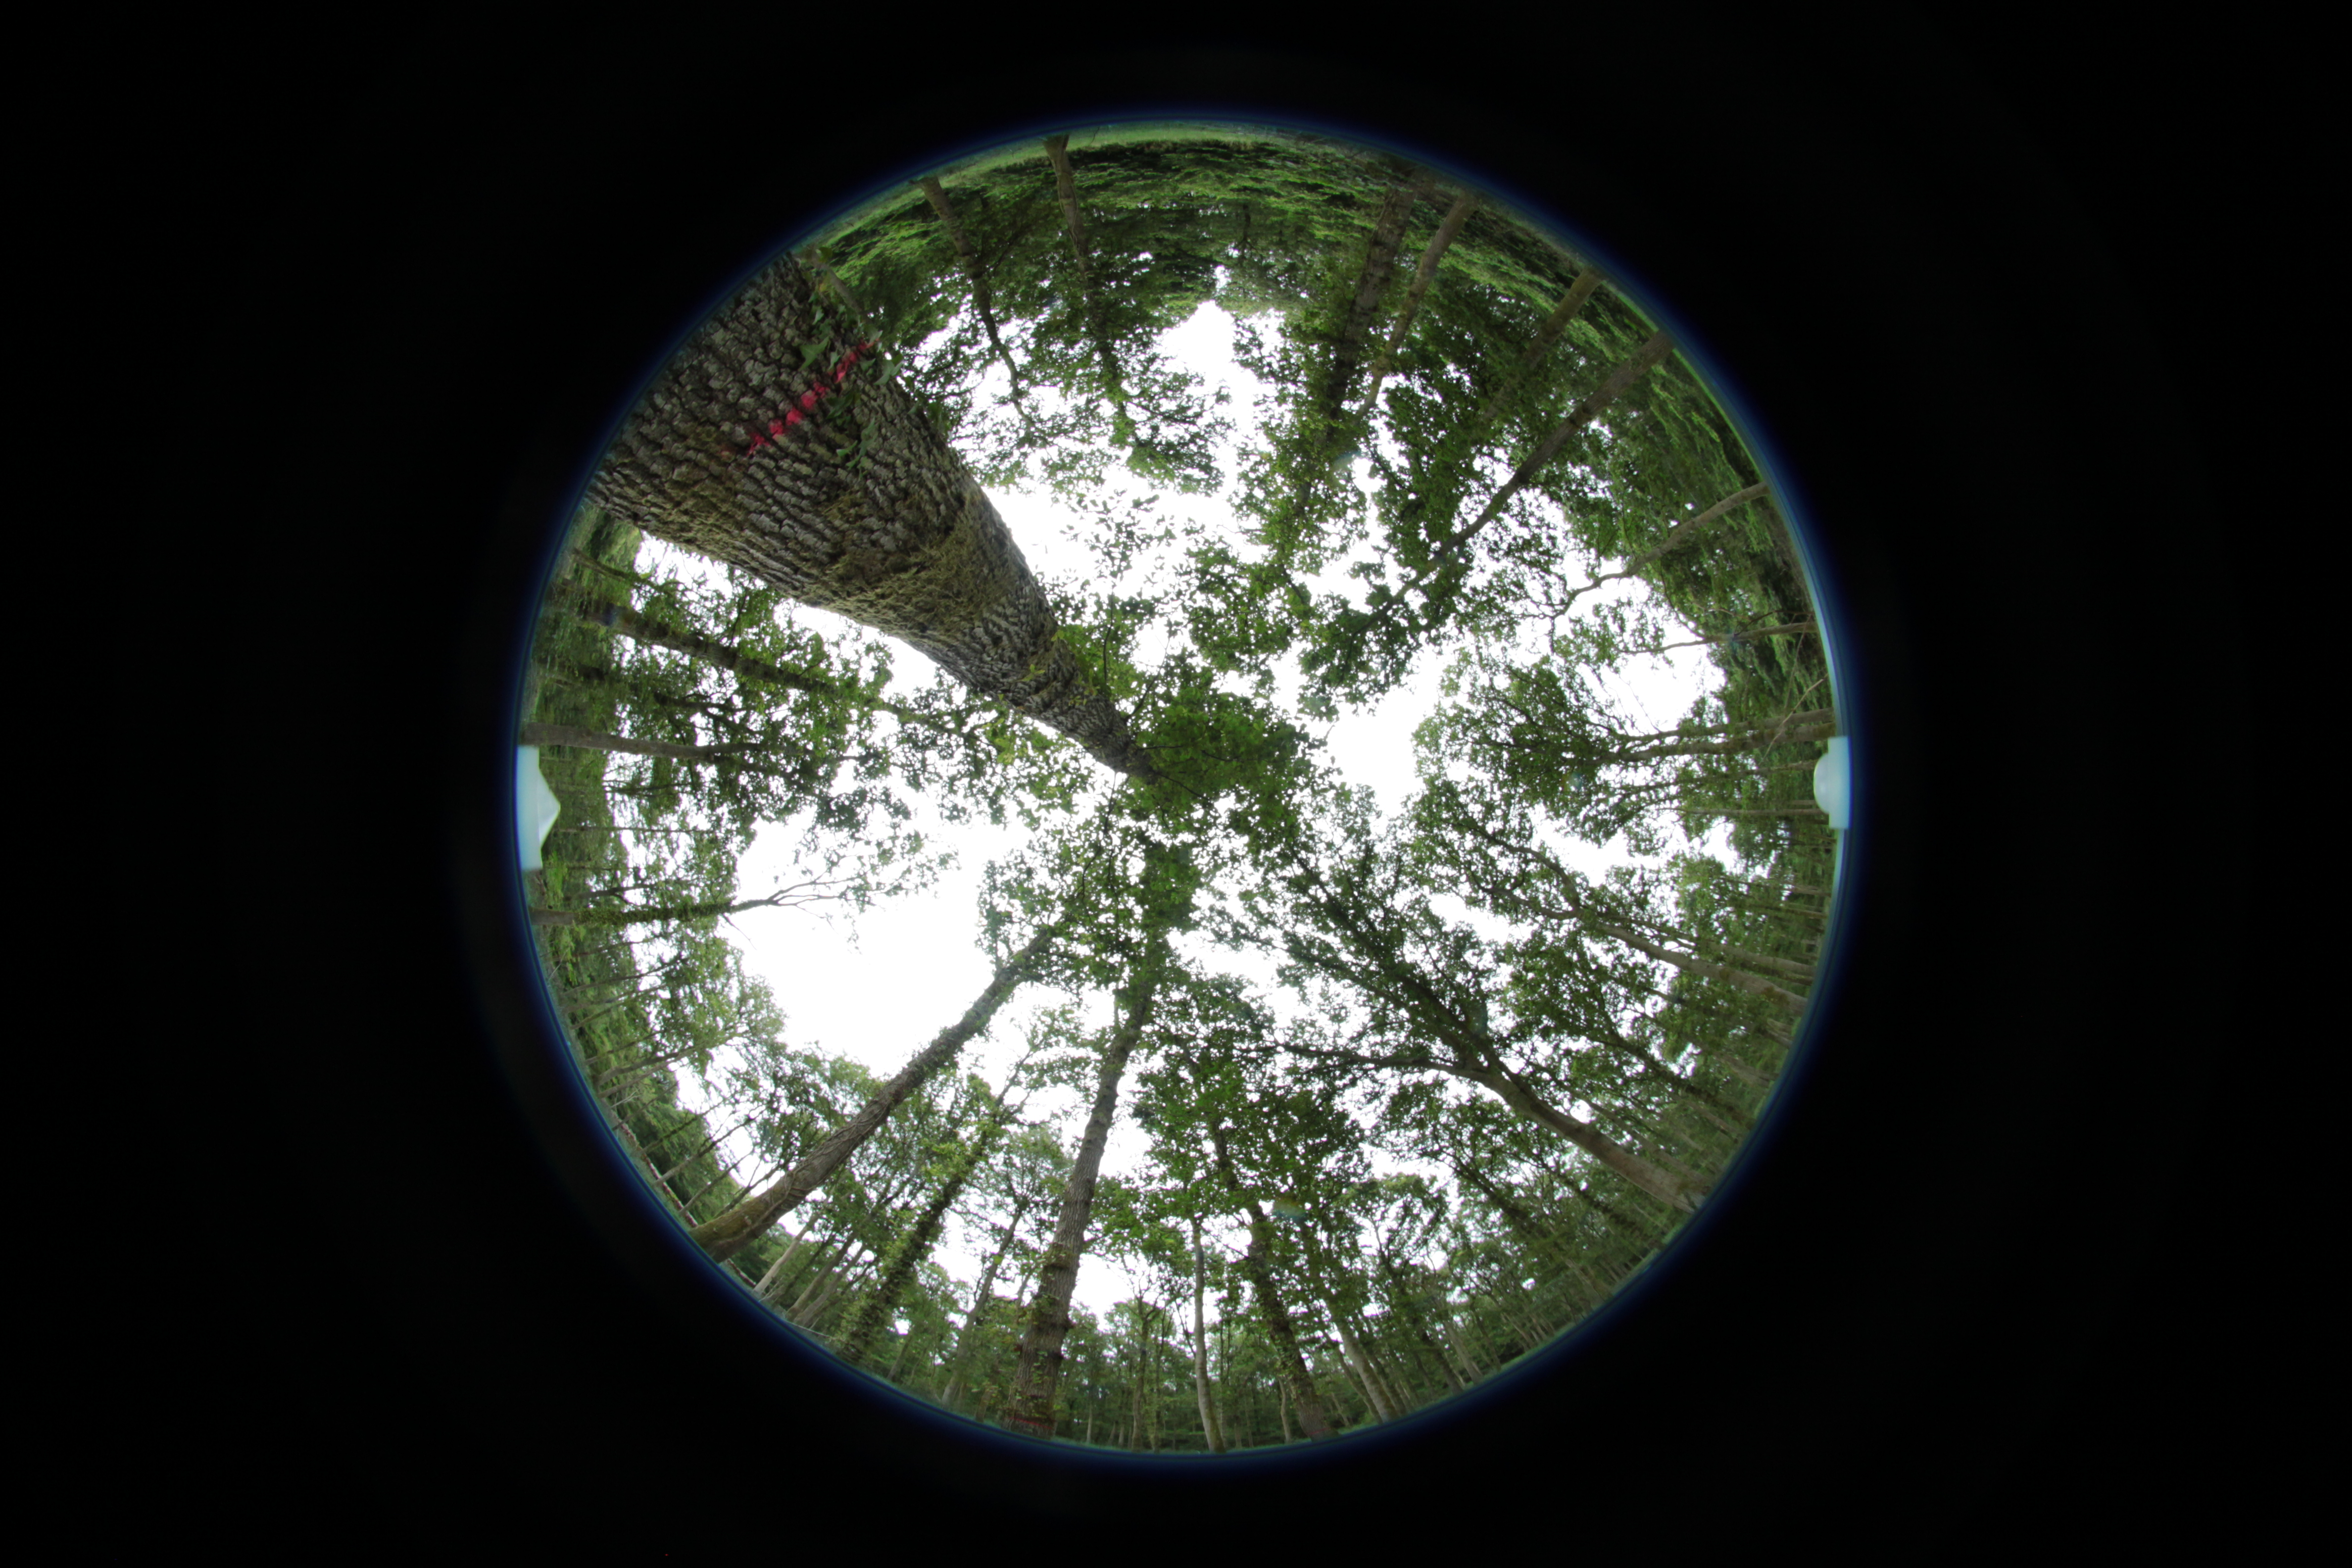
\includegraphics[width=.9\linewidth]{252exp1.jpg}
  \caption{Thinned forest}
  \label{fig:sub2}
\end{subfigure}
\caption{Hemispherical photographs from the Alice Holt flux site showing the difference between the thinned and unthinned sides of the forest.}
\label{fig:hemiphotos}
\end{figure}

\subsection{Litter traps}

\begin{figure}[ht]
    \centering
    \includegraphics[width=0.8\textwidth]{litter_trap.pdf}
    \caption{Litter trap locations for Alice Holt.} \label{fig:lit_traps}
\end{figure}


\subsection{Comparison of methods}

Although the ceptometer is the fastest method to measure LAI it is also the most variable, being extremely sensitive to solar zenith angle and clear sky conditions. If the sun is low in the sky the radiation will pass through much more photosynthetically active material than if the sun is directly above head.

\begin{figure}[ht]
    \centering
    \includegraphics[width=0.8\textwidth]{thinned07.pdf}
    \caption{LAI comparison for unthinned forest.} \label{fig:lai_comp07}
\end{figure}

\begin{figure}[ht]
    \centering
    \includegraphics[width=0.8\textwidth]{thinned14.pdf}
    \caption{LAI comparison for thinned forest.} \label{fig:lai_comp14}
\end{figure}

\section{Point-centred quater observations}

\begin{figure}[ht]
    \centering
    \includegraphics[width=0.8\textwidth]{dbh_me.pdf}
    \caption{Taking diameter at breast height measurements at Alice Holt.} \label{fig:dbh_me}
\end{figure}

\section{Flux tower observations and data processing}

\begin{figure}[ht]
    \centering
    \includegraphics[width=0.8\textwidth]{top_of_flux.pdf}
    \caption{At the top of the Alice Holt flux tower.} \label{fig:flux_me}
\end{figure}

\bibliography{../PhD}{}
\end{document}